\documentclass[runningheads]{llncs}
\usepackage[left=1in,top=1in,right=1in,bottom=1in]{geometry}
\usepackage[T1]{fontenc}
\usepackage[utf8]{inputenc}
\usepackage{amsmath,amssymb,graphicx,xcolor,placeins,float,needspace}
\usepackage[colorlinks=true,linkcolor=blue,citecolor=black,urlcolor=blue]{hyperref}
% RECOMB text-size floor: keep abstract, captions, tables and notes at 10pt.
\let\small\normalsize
\let\footnotesize\normalsize
\DeclareRobustCommand{\moakey}[2]{\textcolor[HTML]{#1}{\rule{0.65em}{0.65em}}\,#2}
\raggedbottom
\setlength{\emergencystretch}{1em}
\renewcommand{\topfraction}{.95}
\renewcommand{\bottomfraction}{.95}
\renewcommand{\textfraction}{.04}
\renewcommand{\floatpagefraction}{.9}
\setcounter{topnumber}{2}
% Compact whole-figure placement; preserve the original composite PDFs.
\setlength{\textfloatsep}{10pt plus 2pt minus 2pt}
\setlength{\intextsep}{10pt plus 2pt minus 2pt}
\setcounter{bottomnumber}{2}
\setcounter{totalnumber}{3}
\expandafter\newcommand\csname captionFigure1\endcsname{\textbf{BioMoAX overview.} (A) Model architecture and five contrastive objectives for learning MOA and compound-identity representations. Colors in the MOA space indicate mechanism groups; positions are schematic. Compound heads use drug measurements only. (B) Retrieval tasks across modalities, batches, cell lines, and perturbation types. Within-cell-line, cross-batch, and cross-cell-line tasks retrieve drugs sharing an MOA. Microscopy images illustrate query and reference inputs.}

\expandafter\newcommand\csname captionFigure2\endcsname{\textbf{Compound identity and MOA retrieval within cell lines.} (A) Same-compound retrieval with disjoint query (20\%) and reference (80\%) crops. Shading shows between-checkpoint SD for BioMoAX and five-split SD for baselines. (B) MOA retrieval with the query compound excluded from the reference library; cross-modal baselines use ridge regression. Error bars show 95\% query-bootstrap CIs; annotations compare BioMoAX with each baseline using Holm-adjusted two-sided Wilcoxon signed-rank tests ($*p<0.05$, $**p<0.01$, $***p<0.001$; ns, not significant, $p\ge0.05$). (C) Image-crop embeddings, with the same annotated crops highlighted across methods. Color denotes MOA, shape distinguishes drugs within each MOA, and gray marks background crops. Two-dimensional maps are fitted independently.}

\expandafter\newcommand\csname captionFigure3\endcsname{\textbf{Cross-batch MOA retrieval and representation structure.} (A) Images of 115 cpg0030 drugs query the cpg0012 reference library for other drugs sharing an MOA; identical-compound matches are absent. Error bars show checkpoint SD for BioMoAX and 95\% query-bootstrap intervals for baselines. Stars show Holm-adjusted two-sided Wilcoxon comparisons with each baseline; thresholds follow Fig.~2. (B) Batch mixing for 32 compounds shared by the two sources; higher normalized scores indicate greater mixing. (C) Two-dimensional distributions of image-crop representations, colored by batch (top) and MOA (bottom). Each point represents a crop; coordinates are identical between the two rows for each method. Gray indicates other or missing MOA annotations.}

\expandafter\newcommand\csname captionFigure4\endcsname{\textbf{Mechanism-related retrieval across cell lines.} (A) Bidirectional U2OS--A549 retrieval in four modality combinations; arrows indicate query-to-reference direction. (B) HT29 images, excluded from image training, query the pooled U2OS/A549 image (I2I) or L1000 expression (I2E) library. In A and B, hits are reference drugs sharing an MOA with the query. Error bars show 95\% query-bootstrap CIs; significance notation follows Fig.~2. (C) Drug-level image representations colored by cell line (top) and MOA (bottom), with shapes denoting cell line. Each point represents an aggregated drug profile; both rows use identical coordinates within each method. Highlighted MOA groups are selected by proximity in the BioMoAX map; gray denotes other drug profiles. Lines connect highlighted profiles sharing an MOA.}

\expandafter\newcommand\csname captionFigure5\endcsname{\textbf{Drug retrieval from CRISPR perturbations.} (A) Retrieval of 1,038 reference drugs using 29 held-out A549 gene perturbations. Positives comprise target-annotated drugs and one-hop MOA neighbors; shading shows 95\% query-bootstrap CIs. (B,C) Selected co-retrieval examples from individual checkpoints: KDR/DDR2--linifanib (B) and ALDH2/AKR1B1--disulfiram (C). Solid pink edges mark the reference-annotated KDR--linifanib and ALDH2--disulfiram pairs; dashed ochre edges mark additional co-retrieval without direct-target annotation. Boxes are enlarged in the adjacent insets; numbers link nodes to image examples.}

\newcommand{\resultfigure}[1]{%
\begin{figure}[!htb]\centering
\includegraphics[width=\linewidth]{figures/fig#1.pdf}
\caption{\csname captionFigure#1\endcsname}\label{fig:#1}
\end{figure}}
\title{BioMoAX: Unified Multimodal Representation Learning for Cellular Perturbation Retrieval}
\titlerunning{BioMoAX}
% Author order and affiliation follow the user-supplied author table.
% Other author contacts retained from that table:
% Yaning Han: yn.han2@siat.ac.cn
% Xuesong Wang: xuesonw@link.cuhk.edu.hk
% Numbered correspondence follows the user-provided template/main.tex example.
\author{Yaning Han\inst{1} \and Xuesong Wang\inst{1} \and Yu Li\inst{1,2} \and Yimin Fan\inst{1,2}}
\authorrunning{BioMoAX}
\institute{The Chinese University of Hong Kong, Hong Kong
\and Correspondence to: liyu@cse.cuhk.edu.hk, fanyimin@link.cuhk.edu.hk}

\begin{document}
\maketitle
\begin{abstract}
Cell morphology and gene expression capture complementary responses to perturbations, but differences in measurement modality and experimental context make mechanism-related cellular responses difficult to compare directly. We present BioMoAX, a multimodal retrieval model trained on Cell Painting images and L1000 expression profiles. Separate projection heads distinguish compound identity from mechanism-of-action (MOA) relationships, with five complementary contrastive objectives using paired measurements, shared MOA annotations and gene--drug associations. The same trained encoders and drug reference library support functional retrieval across measurement modalities, experimental batches, cellular backgrounds and perturbation types. HT29 images excluded from image training achieve Top-5 MOA hit rates of 21.78\% for image-to-image retrieval and 18.69\% for image-to-expression retrieval, compared with 8.45\% and 5.35\% for the strongest corresponding baselines, CellProfiler and ridge-mapped CLOOME. CRISPR image queries for held-out genes achieve a Top-10 hit rate of 19.77\%, compared with 13.79\% for CellProfiler. Two literature-supported co-retrieval cases connect functionally related genes through shared drugs, illustrating how phenotypic references complement incomplete annotations. BioMoAX enables images of drug-treated cells to query existing morphological and expression profiles and CRISPR images to retrieve functionally related drugs.

\par\medskip
\par\smallskip
\noindent\textbf{Code availability.} BioMoAX code is available at \url{https://github.com/YaningHan/BioMoAX}.
\end{abstract}
\clearpage
\section{Introduction}
Cellular responses to drug treatments and genetic perturbations provide an experimental basis for comparing drug mechanisms and gene functions. The Connectivity Map linked perturbations with similar effects through transcriptional signatures~\cite{lamb2006}, and L1000 expanded the scale of expression profiling~\cite{subramanian2017}. Cell Painting records changes in cellular structure and morphology through multiplexed imaging, providing information complementary to expression profiles~\cite{bray2016,way2022}. These measurements allow researchers to search for functionally related drugs or genetic perturbations from their cellular responses. However, the same biological process can produce different responses across measurement modalities and cellular backgrounds, while experimental batches also affect similarities between profiles. Functional retrieval therefore requires identifying features of perturbation responses that connect measurements across these conditions.

CellProfiler extracts morphological features~\cite{stirling2021}, and DeepProfiler learns image representations~\cite{moshkov2024}. Multimodal methods incorporate additional information: CLOOME pairs images with chemical structures~\cite{sanchez2023}, while Semi-Clipped and TIDE transfer information between morphology and expression through cross-modal distillation~\cite{bendidi2025,chen2026}. Pairing images and expression profiles establishes correspondence between measurements of the same drug. Biological text and annotations additionally provide functional information about perturbations, as used by CellCLIP, MorphoCLIP and annotation-informed contrastive learning~\cite{lu2025,ilyosbekov2026,pwesombo2025}. Genetic imaging and matched chemical--genetic screens provide links between gene perturbations and drug responses~\cite{rohban2017,chandrasekaran2024}, allowing gene-function findings and chemical interventions to inform each other~\cite{li2026unipert}. For retrieval across these settings, representations should retain same-drug correspondence and connect different drugs and genetic perturbations by function.

To combine measurement pairing with functional associations, we present BioMoAX, which learns cellular perturbation representations from Cell Painting images, L1000 expression profiles, and chemical--genetic image pairs through five complementary contrastive objectives. In a separate compound projection space, the compound-paired objective aligns images and expression profiles of the same drug to learn cross-modal identity correspondence. In a shared functional projection space, image MOA and expression MOA objectives connect drugs with shared mechanisms within each modality, while a cross-modal MOA objective connects mechanism-related drugs across modalities. A gene--drug paired objective uses CRISPR and associated drug image pairs to incorporate genetic perturbations into this functional space. By separating compound identity from perturbation function and jointly modeling within-modality, cross-modal, and chemical--genetic relationships, BioMoAX supports retrieval of functionally related responses across measurement modalities and perturbation types (Fig.~1A).

We evaluated compound identity and within-cell-line MOA retrieval before extending queries across experimental batches, cell lines and perturbation types (Fig.~1B). In bidirectional U2OS--A549 retrieval, image queries identified mechanism-related image and expression profiles from the other cell line. HT29 images excluded from image training queried the U2OS/A549 library, achieving image-to-image (I2I) and image-to-expression (I2E) Top-5 MOA hit rates of 21.78\% and 18.69\%, compared with 8.45\% for CellProfiler and 5.35\% for ridge-mapped CLOOME, the strongest corresponding baselines. The I2E queries crossed both cellular background and measurement modality, using existing transcriptomic profiles as references for image-only queries. CRISPR queries for held-out genes achieved a Top-10 hit rate of 19.77\%, compared with 13.79\% for CellProfiler. KDR and DDR2 perturbations co-retrieved linifanib, while ALDH2 and AKR1B1 perturbations co-retrieved disulfiram. In both cases, the retrieved drug connects a reference-annotated gene--drug pair with an additional association supported by independent literature~\cite{karaman2008,yoshino2020npl4}.

\resultfigure{1}
\section{Methods}
\subsection{Data and splits}
We used Cell Painting Gallery data~\cite{weisbart2024}: cpg0012 (U2OS) and cpg0004 (A549) for drug image--expression learning, cpg0016 (A375/MCF7) for additional training, and cpg0000 for chemical--genetic alignment. Additional cpg0030 images from 154 training records were used for image-based supervision; the 115 cpg0030 retrieval queries were excluded from training. Drug records were partitioned separately by source and cell line, giving 473 training/90 query records in U2OS and 738/301 in A549. The cpg0000 data contain 130 genes and 260 compound records per cell line; a shared gene-level split assigns 90 genes to training and 40 to evaluation.

\subsection{Model architecture}
\noindent\textbf{Image encoder.} A shared ViT~\cite{dosovitskiy2021} encodes drug and CRISPR images (Fig.~1A). Each five-channel $128\times128$ Cell Painting crop is divided into $16\times16$ patches and embedded as 384-dimensional tokens. The encoder has 12 Transformer blocks, each with six attention heads. Two independent two-layer MLP projection heads~\cite{chen2020simclr} map the final 384-dimensional CLS token to normalized 256-dimensional embeddings. The compound head is used for drug identity matching and the MOA head for functional retrieval. CRISPR images use the MOA head.

\noindent\textbf{Expression encoder.} An MLP with hidden dimensions of 1,024 and 512 encodes each 12,328-dimensional L1000 profile. Both layers use layer normalization, GELU activation, and dropout. Separate two-layer compound and MOA projection heads map the 512-dimensional representation to normalized 256-dimensional embeddings. These heads do not share parameters with the image heads.

\Needspace{30\baselineskip}
\subsection{Supervision and training objectives}
\begingroup
\setlength{\parskip}{5pt}
\setlength{\parindent}{0pt}
Let $Z^{I,c}$ and $Z^{E,c}$ denote image and expression embeddings in the compound space, and $Z^{I,m}$ and $Z^{E,m}$ those in the MOA space. For normalized embeddings $A=\{a_i\}$ and $B=\{b_j\}$ and a positive mask $P$, the directed contrastive loss is

\begin{equation}
\begin{aligned}
\ell(A\!\to\!B;P)
&=-\frac{1}{|\mathcal V|}
\sum_{i\in\mathcal V}\frac{1}{\max(1,\sum_jP_{ij})}\\[3pt]
&\qquad{}\times\sum_j P_{ij}
\log\frac{\exp(a_i^\top b_j/\tau)}
{\sum_{k\in\mathcal B(i)}\exp(a_i^\top b_k/\tau)}.
\end{aligned}
\label{eq:contrastive}
\end{equation}

Here $\tau$ is a learned temperature, $\mathcal B(i)$ is the candidate set, and $\mathcal V$ is the anchor set. Cross-group alignment uses the bidirectional form~\cite{radford2021}:

\begin{equation}
\mathcal C(A,B;P)=\frac12
\bigl[\ell(A\to B;P)+\ell(B\to A;P^\top)\bigr].
\label{eq:bidirectional}
\end{equation}
Within-modality supervised contrastive learning~\cite{khosla2020}, denoted $\mathcal S(Z;P)$, excludes self-comparisons. The following five objectives correspond to Fig.~1A.

\Needspace{8\baselineskip}
\textbf{Compound-paired supervision ($L_1$).}
Paired image and expression records of the same drug are positives. This objective learns identity correspondence in the compound space:

\begin{equation}
P^c_{ij}=\mathbf1[i=j],
\qquad L_1=\mathcal C(Z^{I,c},Z^{E,c};P^c).
\label{eq:compound-pair}
\end{equation}
\Needspace{12\baselineskip}
\textbf{Within-modality MOA supervision ($L_2$ and $L_3$).}
Let $\mathcal M_i$ be the MOA annotation set of drug $i$. Different records sharing at least one MOA are positives, allowing multiple positives per anchor. Image and expression objectives organize functional relationships within their respective modalities:

\begin{equation}
\begin{aligned}
P^m_{ij}&=\mathbf1[i\ne j]\,
          \mathbf1[\mathcal M_i\cap\mathcal M_j\ne\varnothing],\\[3pt]
L_2&=\mathcal S(Z^{I,m};P^{m,I}),\\[3pt]
L_3&=\mathcal S(Z^{E,m};P^{m,E}).
\end{aligned}
\label{eq:within-moa}
\end{equation}
\Needspace{10\baselineskip}
\textbf{Cross-modal MOA supervision ($L_4$).}
Shared MOA annotations connect image and expression records, including records of different drugs:

\begin{equation}
\begin{aligned}
P^\times_{ij}&=\mathbf1[\mathcal M_i\cap\mathcal M_j\ne\varnothing],\\[3pt]
L_4&=\mathcal C(Z^{I,m},\operatorname{sg}(Z^{E,m});P^\times).
\end{aligned}
\label{eq:cross-moa}
\end{equation}
Here $\operatorname{sg}$ stops gradients to the expression branch for this term.

\Needspace{9\baselineskip}
\textbf{Gene--drug supervision ($L_5$).}
For each sampled training gene, a CRISPR image is paired with an associated drug image from the same cell line. Their embeddings $Z^{G,m}$ and $Z^{D,m}$ share the image encoder and MOA head. A sampled-pair mask connects genetic and chemical perturbations:

\begin{equation}
P^g_{ij}=\mathbf1[i=j],
\qquad L_5=\mathcal C(Z^{G,m},Z^{D,m};P^g).
\label{eq:gene-drug}
\end{equation}
\Needspace{6\baselineskip}
The five objectives are jointly optimized with fixed weights:

\begin{equation}
\mathcal L=2L_1+1.7L_2+3L_3+2L_4+L_5.
\label{eq:five-losses}
\end{equation}

Image crops are normalized channel-wise. We use AdamW~\cite{loshchilov2019}, a learning rate of $10^{-4}$, weight decay of $10^{-2}$, and cosine decay after warm-up.
\endgroup

\subsection{Baselines and retrieval evaluation}
We compare CellProfiler~\cite{stirling2021}, which extracts morphological features; DeepProfiler~\cite{moshkov2024}, which learns image features; CLOOME~\cite{sanchez2023}, trained on image--chemical structure pairs; and CellCLIP~\cite{lu2025}, trained to align images with perturbation-related text. CLOOME and CellCLIP use pretrained representations; raw L1000 profiles provide the expression baseline.

Table~\ref{tab:model-size} summarizes the image feature extractors and their parameter counts.

\begin{table}[!htb]
\caption{Image feature extractors and parameter counts.}
\label{tab:model-size}
\centering
\setlength{\tabcolsep}{0pt}
\renewcommand{\arraystretch}{1.22}
\begin{tabular*}{\linewidth}{@{}l@{\hspace{1.5em}}l@{\extracolsep{\fill}}r@{}}
\hline
Method & Image feature extractor & Parameters (M) \\
\hline
BioMoAX & ViT + one projection head & 22.04 \\
CellProfiler & Handcrafted morphological features & -- \\
DeepProfiler & EfficientNet-B0 & 4.01 \\
CLOOME & Five-channel ResNet-50 & 24.56 \\
CellCLIP & DINOv2-G + channel Transformer & 1,477.26 \\
\hline
\end{tabular*}
\par\vspace{4pt}
\raggedright
Image inference parameters, including frozen weights; --, no neural encoder.
\end{table}


We denote image and expression modalities by I and E. Retrieval directions are I2I (image-to-image), E2E (expression-to-expression), I2E (image-to-expression), and E2I (expression-to-image), with the first modality specifying the query and the second the reference library. For image retrieval, we average up to 100 normalized crop embeddings per condition~\cite{ljosa2013} and renormalize. References are ranked by cosine similarity to the query. Top-$K$ hit rate is the percentage of queries with at least one positive among their first $K$ results. In MOA retrieval, positives share an MOA with the query; the query drug is excluded in within-cell-line MOA searches.

For image baselines not aligned with L1000, we fit ridge regression on paired profiles from the pooled U2OS/A549 training set. Both input and target features are standardized using their training means and standard deviations. The mapping is learned by

\begin{equation}
(W^*,b^*)=\arg\min_{W,b}
\left\|XW+\mathbf1 b^\top-Y\right\|_F^2
+\alpha\|W\|_F^2,\qquad \alpha=1.
\label{eq:ridge}
\end{equation}

Here $X$ and $Y$ contain paired standardized training profiles in the source and target modalities, $W$ is the mapping matrix, $b$ is the intercept, and $\mathbf1$ is a vector of ones. The first term measures mapping error; the second penalizes large coefficients. I2E and E2I mappings are fitted independently. Standardization and mappings remain fixed during evaluation; mapped queries are ranked against standardized target-modality references by cosine similarity.

\section{Results}
\subsection{Retrieval of compound identity and mechanism of action}
Recognizing the same drug requires reproducible identity features, whereas connecting different drugs sharing an MOA requires functional similarity. A retrieval framework should preserve both relationships across morphology and expression. We evaluated same-drug identity in U2OS and A549 (Fig.~2A), then excluded query-drug matches to assess within- and cross-modal MOA retrieval (Fig.~2B), alongside local image neighborhoods (Fig.~2C).

\resultfigure{2}

The compound head identified the same drug across crops (Fig.~2A). U2OS Top-1 hit rates were 99.19\% for BioMoAX and 96.22\% for CellCLIP, both near the task ceiling. In A549, BioMoAX achieved 92.00\%, versus 72.23\% for CLOOME.

Excluding same-drug matches, BioMoAX retrieved other compounds sharing an MOA (Fig.~2B). CellCLIP had higher I2I means in both cell lines, but differences were not significant. BioMoAX matched raw L1000 in U2OS E2E at 22.22\% and exceeded it in A549 (20.60\% versus 17.94\%).

BioMoAX\textquotesingle s main advantage is cross-modal functional matching: connecting mechanism-related morphology and expression responses in a common MOA space enables reciprocal retrieval. This advantage is clearer in A549, where BioMoAX\textquotesingle s I2E Top-5 hit rate was 12.29\%, versus 8.11\% for ridge-mapped CellCLIP, and E2I was 16.94\%, versus 13.29\% for ridge-mapped CellProfiler, the strongest corresponding baselines.

In A549, BioMoAX and CellProfiler had similar I2I performance but different I2E hit rates (12.29\% and 6.31\%). CellCLIP had higher I2I means yet lower means in both cross-modal directions. These comparisons distinguish image-only mechanism discrimination from morphology--expression matching, consistent with directly learning functional correspondence. Relative to baselines, cross-modal gains are concentrated in A549 and cover both image-to-expression and expression-to-image retrieval.

Figure~2C compares local neighborhoods of the same highlighted crops across methods. In several BioMoAX neighborhoods, responses to different drugs sharing an MOA overlap, forming multi-compound functional neighborhoods. This complements retrieval with same-drug matches excluded: the framework retains drug identity and connects related responses across compounds in the MOA space, supporting queries between morphology and expression.

\subsection{Mechanism-related retrieval across experimental batches}
Experimental protocols and imaging conditions can shift representations across sources, obscuring functional similarities. We tested whether an existing library supports queries from another source, using cpg0030 images to query cpg0012. All 115 queries have other reference drugs sharing an MOA but no identical-compound matches, requiring matching across sources and compound identities (Fig.~3A).

\begin{figure}[!htb]
\centering
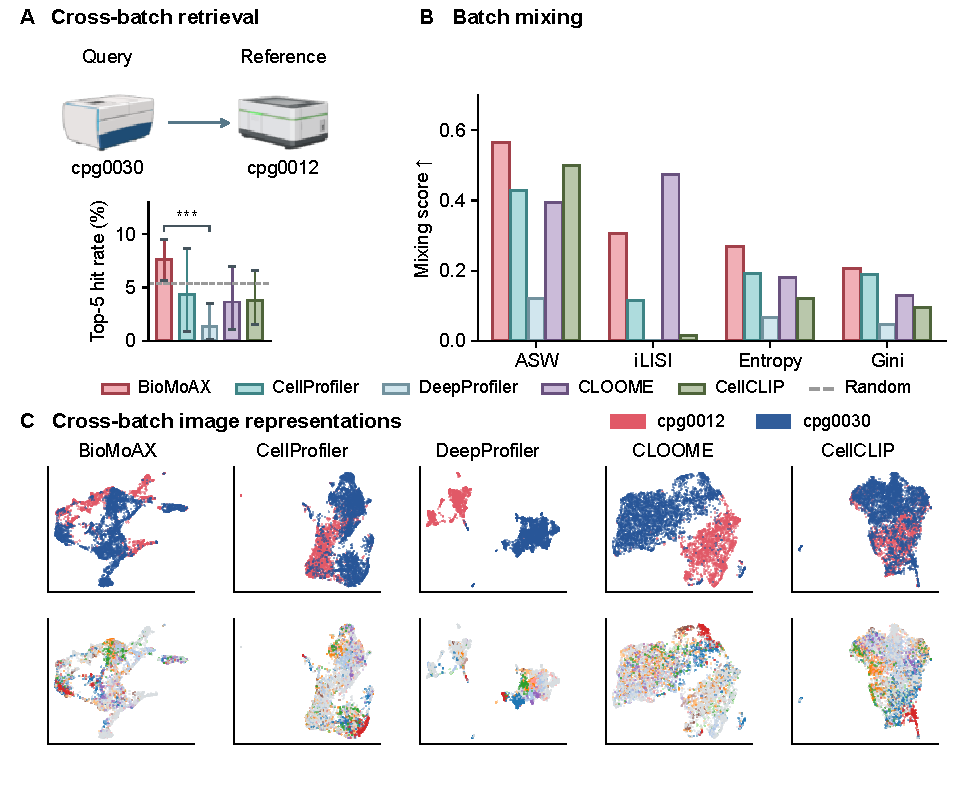
\includegraphics[width=\linewidth]{figures/fig3.pdf}
\caption{\csname captionFigure3\endcsname}\label{fig:3}
\end{figure}

Top-5 hit rates were 7.59\% for BioMoAX, 4.35\% for CellProfiler, 1.39\% for DeepProfiler, 3.65\% for CLOOME and 3.83\% for CellCLIP, with a 5.37\% random reference. BioMoAX had the highest mean; only its difference from DeepProfiler was significant after correction of paired Wilcoxon tests. Retrieved positives connect different compounds, showing that functional information remains retrievable across sources. Limited absolute hit rates leave substantial room for improvement.

For 32 shared compounds, mixing was assessed with drug identity held constant (Fig.~3B). In the displayed comparison, BioMoAX had the highest ASW, entropy and Gini scores; CLOOME had the highest iLISI. Crop-level maps show partial source overlap for BioMoAX, CellProfiler and CellCLIP, versus more pronounced separation for DeepProfiler (Fig.~3C). Mixing evaluates same-drug similarity across sources; MOA retrieval tests functional relationships between different drugs. Together, these analyses assess whether source-related separation can be reduced while preserving information that distinguishes and connects drug responses. The results support reusing existing measurements for mechanism-related queries from another experimental source.

\subsection{Mechanism-related retrieval across cellular backgrounds}
Cell lines differ in their basal states and drug sensitivities, so perturbations sharing an MOA may induce different morphological and transcriptional responses. A useful functional reference should recognize related responses across these backgrounds and remain usable when a query cell line has not contributed to image training. We first evaluated bidirectional retrieval between U2OS and A549, using one cell line to query the other's library for drugs sharing an MOA in all four modes: I2I, E2E, I2E and E2I (Fig.~4A).

\resultfigure{4}

BioMoAX had higher means than the corresponding CellProfiler, DeepProfiler and raw L1000 baselines in both query directions. Its U2OS-to-A549 I2I mean was close to CellCLIP (15.93\% versus 15.56\%), while its cross-modal means exceeded CellCLIP in both directions. For example, A549 images retrieved U2OS expression profiles with a Top-5 mean of 20.10\%, compared with 7.78\% for both ridge-mapped CellProfiler and CellCLIP. Thus, image queries could identify mechanism-related responses in another cell line through either morphology or expression, supporting functional comparisons despite changes in cellular background. The two cross-modal directions further allow either images or expression to query the learned functional space, with measurements from another cell line providing the reference.

The shared-MOA criterion permits responses that differ across cell lines to be compared on the basis of annotated function. Successful retrieval therefore reflects a recognizable functional relationship across backgrounds without requiring identical morphological or transcriptional profiles.

U2OS and A549 were represented during training. To test use of the reference library beyond these image-training backgrounds, we next queried it with HT29 images, reusing the trained encoders and MOA heads. HT29 drug images searched the pooled U2OS/A549 library, achieving an I2I Top-5 mean of 21.78\%, compared with 8.45\% for CellProfiler, the strongest baseline (Fig.~4B). The reference collection could therefore support morphological queries from an additional cell line without training a separate HT29 image encoder.

HT29 images also retrieved reference transcriptional responses. The I2E Top-5 mean was 18.69\%, compared with 5.35\% for the strongest baseline, ridge-mapped CLOOME. Here, the queries contained only HT29 images and the references were U2OS/A549 L1000 profiles, crossing cellular background and measurement modality simultaneously. This setting is relevant when imaging is available for a new cellular background but matched expression measurements are not: existing transcriptomic collections can serve as functional references for interpreting the image responses. Responses from related reference treatments could then provide transcriptional context for hypothesis generation and follow-up in the query cell line.

The representation maps provide spatial context for these comparisons (Fig.~4C). The same aggregated drug profiles are colored by cell line and MOA. Some BioMoAX neighborhoods contain profiles from different drugs and cell lines sharing an MOA. CellProfiler also shows cross-cell-line mixing, whereas DeepProfiler separates the cell lines more strongly. The MOA view relates the illustrated cross-cell overlap to annotated functional relationships.

\FloatBarrier
\subsection{Functional relationships between genetic and chemical perturbations}
Genetic and chemical screens investigate cellular function from complementary perspectives: the former identify genes involved in cellular processes, whereas the latter seek chemical interventions that modulate cellular states. Connecting the two enables gene-function information and drug-induced responses to inform each other~\cite{li2026unipert}. A shared representation further allows an existing drug collection to serve as a common reference linking genetic findings to chemical interventions. We therefore used A549 CRISPR images of held-out genes to query the same drug reference library, evaluating functional retrieval across perturbation types (Fig.~5).

\begin{figure}[!htb]
\centering
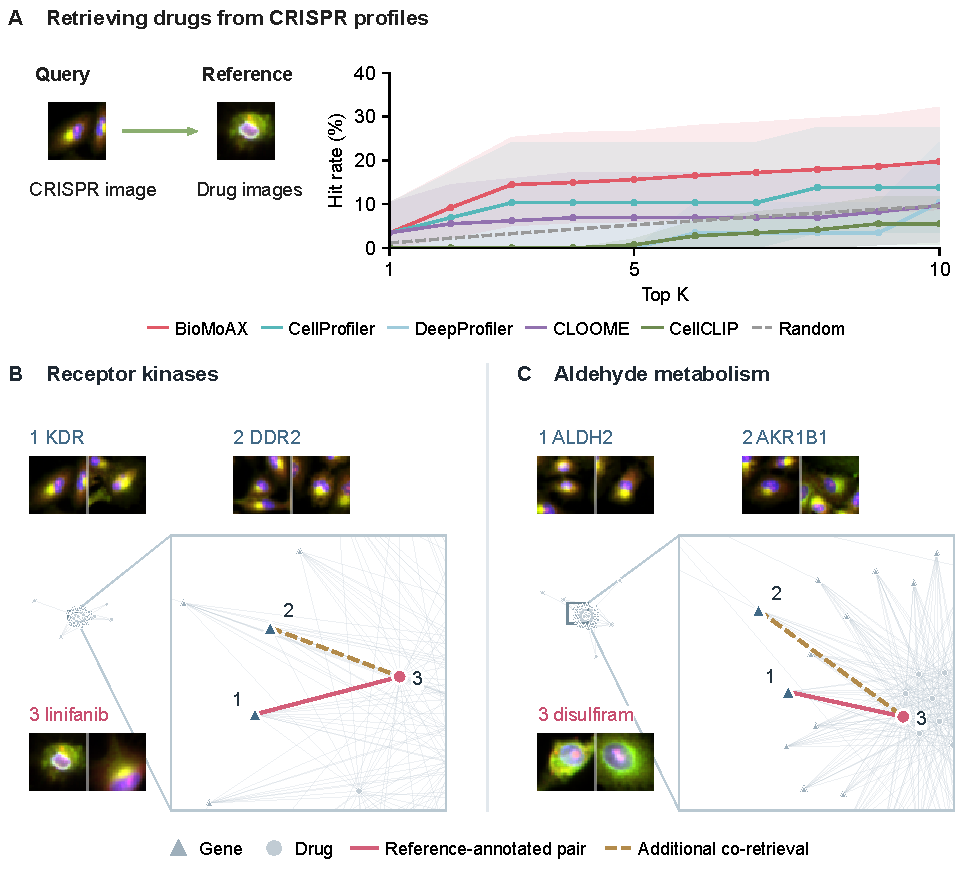
\includegraphics[width=\linewidth]{figures/fig5.pdf}
\caption{\csname captionFigure5\endcsname}\label{fig:5}
\end{figure}

Across 29 eligible gene queries and 1,038 reference drugs, BioMoAX achieved a Top-10 hit rate of 19.77\%, compared with 13.79\% for CellProfiler, the strongest baseline at this depth (Fig.~5A). This result extends the preceding drug-to-drug functional retrieval to genetic perturbations, connecting morphological responses of genes unseen during training to the drug reference library.

Perturbations of the receptor tyrosine kinases KDR and DDR2 both retrieved linifanib (Fig.~5B). KDR--linifanib is reference-annotated, with biochemical and cellular evidence supporting inhibition~\cite{albert2006}. An independent kinase screen also reported linifanib binding to DDR2, although this pair is absent from the current reference annotations~\cite{karaman2008}. Co-retrieval thus recovered an experimentally supported pharmacological relationship beyond the reference annotations, demonstrating how the shared representation can complement incomplete annotation.

The second example involves the aldehyde-metabolism genes ALDH2 and AKR1B1, which participate in oxidative and reductive metabolism of reactive aldehydes, respectively~\cite{chen2008aldh2,srivastava1998hne}. Both retrieved disulfiram (Fig.~5C). Experimental studies support inhibition of ALDH2 by disulfiram and its metabolites~\cite{lam1997disulfiram}; another study observed decreased AKR1B1 protein levels after disulfiram treatment in renal carcinoma xenografts~\cite{yoshino2020npl4}.

The two cases involve receptor tyrosine kinases and aldehyde-metabolism genes, respectively, illustrating the use of a shared drug as a phenotypic reference. Each case links a reference-annotated gene--drug pair to a second gene--drug association absent from the current reference annotations; independently reported drug binding or post-treatment protein changes provide biological support for these relationships. The shared space can therefore use existing drug responses to bring functionally related genetic perturbations into a common comparison framework, extending functional comparisons beyond current annotations.

\FloatBarrier
\section{Discussion}
BioMoAX organizes morphology, expression and genetic perturbation data within a unified retrieval framework, allowing the same encoders and drug reference library to support functional comparisons across modalities, experimental sources, cellular backgrounds and perturbation types. In A549, methods ranked differently in image-to-image and cross-modal MOA retrieval; BioMoAX showed its clearest advantage in functional matching between morphology and expression. Compound pairing provides identity correspondence between measurements, while shared MOAs and gene--drug associations supervise functional relationships across perturbations. This design allows jointly trained representations to retain drug identity and connect mechanism-related perturbations, providing a common functional reference for multiple query tasks.

This reference-based approach is useful when measurements are incomplete across experiments. When only imaging is available for a cellular background, cross-cell-line image-to-expression retrieval can identify mechanism-related responses in existing transcriptomic collections, informing pathway hypotheses and follow-up validation. Genetic queries extend this use to gene-function studies: existing drug responses provide a common reference for comparing gene perturbations and connecting genetic-screen findings to specific chemical interventions. Independent literature supporting the two co-retrieval cases shows how this reference can complement relationships absent from current gene--drug annotations. Existing morphology, expression and drug measurements can thus remain useful in subsequent experiments, providing a comparable functional context for further queries.

Current evaluation is limited by cellular backgrounds, genetic perturbation numbers, and annotation coverage. Crop averaging loses cellular heterogeneity, while dose and exposure time remain unmodeled. Broader gene and compound coverage and representations retaining cellular variation should clarify how functional relationships vary across doses, times, and backgrounds. Genetic and chemical perturbation experiments testing shared downstream responses would clarify the biological basis and scope of these retrieval relationships.


\clearpage
\bibliographystyle{splncs04}
\bibliography{references}
\clearpage
\appendix
\section{Implementation and evaluation details}\label{app:protocol}
\textbf{Supervision implementation.} A drug record is a compound entry within a source and cell line. MOA masks are constructed within each sampled batch; unannotated drugs can still contribute to compound pairing. For cpg0000 compounds, MOA is assigned as the most frequent reference MOA among drugs targeting the associated gene. $L_1,L_2,L_3,L_4$ have separate learned temperatures; $L_5$ shares the $L_2$ temperature. Only these five objectives are active. Within-modality losses average over anchors with positives; cross-group losses average over all anchors, with zero contribution from anchors without positives.

\textbf{Retrieval settings.} Same-compound retrieval uses the compound head, with five random 20\% query/80\% reference crop splits. Functional retrieval uses MOA heads and excludes the query drug in within-cell-line and cross-batch MOA searches. U2OS and A549 query each other's reference libraries. Cross-batch retrieval uses 115 cpg0030 queries and 690 cpg0012 references; cpg0030 queries are excluded from encoder training. Batch mixing uses 32 shared compounds. HT29 images are excluded from training; 71 drug queries search 1,729 pooled U2OS/A549 records. CRISPR retrieval uses 29 of the 40 held-out A549 genes with positives among 1,038 reference drugs. Positives are annotated target drugs plus drugs sharing an MOA with those drugs, expanded once. Functional queries must have at least one positive.

\textbf{Metrics and statistics.} Random rates use query-specific library sizes and positive counts. Batch-mixing scores are ASW, iLISI, Leiden-cluster entropy and normalized Gini, oriented so that higher is better; panel-specific settings are stated in captions.

Query-bootstrap 95\% CIs use the 2.5th/97.5th percentiles, averaging repeated hit indicators within each query first; models and libraries are fixed. Panels showing standard deviations are identified in captions. Figs.~2B, 3A and 4 use paired-query two-sided Wilcoxon signed-rank tests: zero differences are discarded, tied absolute differences receive average ranks, and exact conditional sign-randomization $p$-values are Holm-adjusted within families of 26, 4 and 52 comparisons, respectively (the last includes both heads). In Fig.~3A, the five crop draws are averaged within each checkpoint and then equally across the three checkpoints for each of the 115 queries; the four tests compare the MOA head with the four displayed baselines. Pratt and paired sign-flip tests provide sensitivity checks.

\textbf{Parameter counting.} Table~\ref{tab:model-size} counts parameters in the image inference path, including frozen weights, with M denoting $10^6$ parameters. BioMoAX includes the shared ViT and one active projection head; its compound and MOA heads have equal sizes. DeepProfiler excludes its unused training classifier. CLOOME includes the image output layer; CellCLIP counts the DINOv2-G backbone once across channels, together with the channel Transformer. Expression, chemical and text encoders, unused heads, non-parameter buffers and ridge mappings are excluded. CellProfiler has no neural image encoder, and raw L1000 expression profiles are not part of this image-side comparison.

\textbf{Representation visualization.} Fig.~2C highlights the same annotated crops across methods, sampling 20 MOAs, four drugs per MOA and three crops per drug. In Fig.~4C, UMAP is fitted on A549 and applied to U2OS and HT29. Seven distant background points are omitted from each BioMoAX and CellProfiler map; all highlighted drug profiles are retained.

\textbf{Case visualization.} Networks in Fig.~5B and C use seed45\_ep028 and seed43\_ep029, respectively. Each network includes all query genes and the union of their Top-10 reference drugs across five crop draws for that checkpoint. Both ALDH2 and AKR1B1 retrieve disulfiram in all five crop draws of seed43, but not among the Top-10 in the other two checkpoints. Disulfiram is also retrieved broadly by other genes in seed43. The examples therefore illustrate shared-drug retrieval, not gene specificity or new direct-target validation. The pink edges indicate the current reference annotations, whose absence for the dashed edges does not establish absence from all literature. External evidence for DDR2--linifanib comes from an in vitro kinase-binding screen~\cite{karaman2008}. The AKR1B1 protein decrease reported by Yoshino et al. was observed in renal carcinoma xenografts and was not reproduced in the same study\textquotesingle s cultured-cell experiments~\cite{yoshino2020npl4}.

\end{document}
